\documentclass{article}
\usepackage[utf8]{inputenc}
\usepackage[backend=biber]{biblatex}
\usepackage{amssymb}
\usepackage{amsmath}
\usepackage{dsfont}
\addbibresource{bib.bib}
\setlength{\parindent}{0em}
\bibliography{bib}
\setlength{\parskip}{6pt}
\usepackage[margin=1.0in]{geometry}
\usepackage{graphicx}
\usepackage{caption}
\usepackage{subcaption}
\usepackage{wrapfig}
\usepackage{url}

\title{Intro to deep learning with PyTorch}
\author{Miguel A. Saavedra-Ruiz}
\date{May 2020}
\linespread{1.0}

\nocite{*}


\begin{document}

\maketitle

\section*{Generative Adversarial Networks (GAN)}

Generative Adversarial Networks (GAN) are an architecture derived from fully connected layers and convolutional neural networks. This sort of networks have the capability to generate new samples similar to the data they were trained on. An example of a GAN would be a generate faces after being trained on a large data-set of real faces. The results of such example can be seen at Fig. \ref{fig:f1}


\begin{figure}[ht]
    \centering
    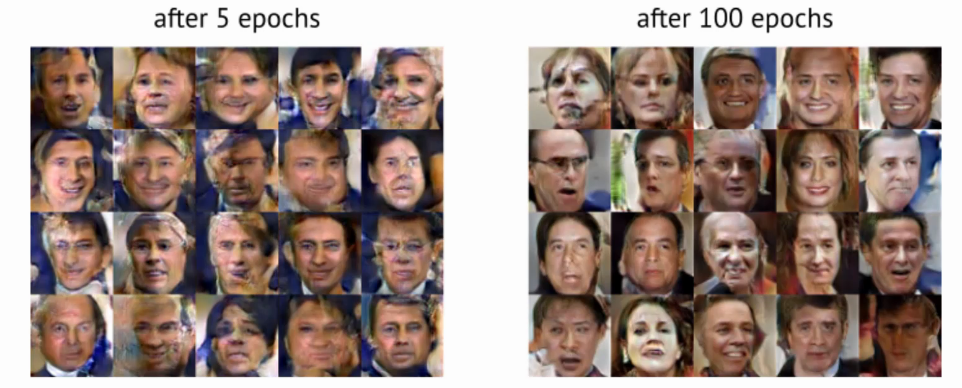
\includegraphics[width=0.65\textwidth,height=0.65\textheight,keepaspectratio]{images/face_generator.png}
    \captionsetup{justification=centering}
    \caption{Generation of faces with GAN}
    \label{fig:f1}
\end{figure}

To understand the general idea of a GAN network it used the concept of two networks, a generator (G) and a discriminator (D). These two networks compete against each other. A simple way to understand a GAN network is use the analogy of the forger and the detective. Imagine a forger trying to forge paintings and make them real enough that the detective won't notice. Here it is possible to think about the forger as a generator and the detective as the discriminator Fig. \ref{fig:f2}.

\begin{figure}[ht]
    \centering
    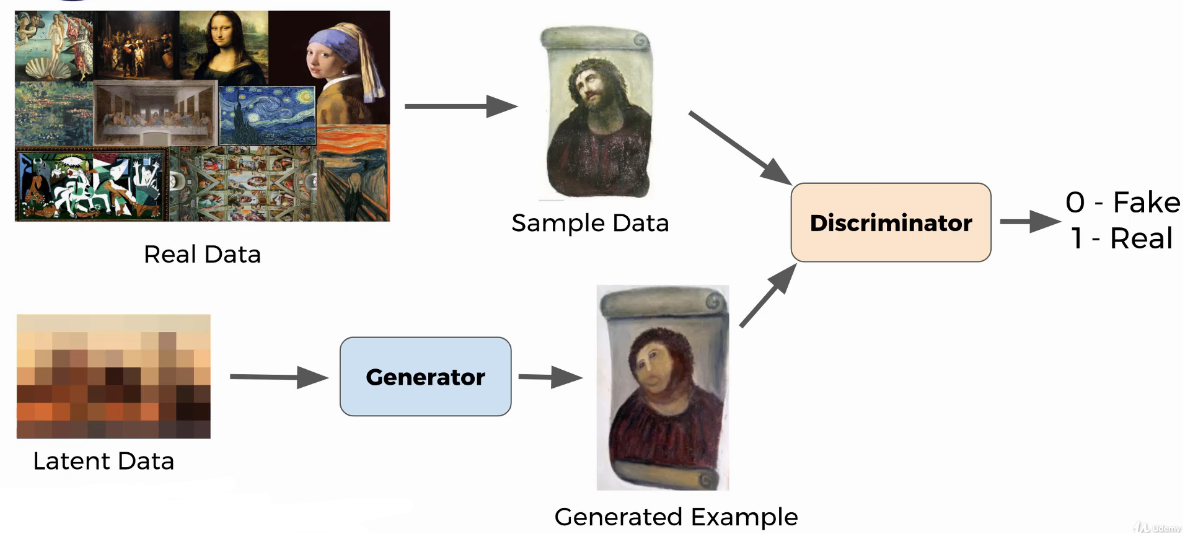
\includegraphics[width=0.7\textwidth,height=0.7\textheight,keepaspectratio]{images/gan.png}
    \captionsetup{justification=centering}
    \caption{GAN architecture}
    \label{fig:f2}
\end{figure}

The generator is represented with a blue box and the discriminator with the orange one. 
The idea behind this architecture is that the generator makes fake data to pass to the discriminator. On the other hand, the discriminator also sees real data such as real images and it predicts if the data received is real or fake. The generator is trained to try to fool the discriminator by making its output data to look as close as possible to real data and the discriminator is trained to figure out which data is real and which data is fake. The final result is the generator learns to make data that is indistinguishable from real data to the discriminator Fig. \ref{fig:f2}.

Latent data is basically random noise that is feed into the generator as an input and this tries to produce an image as similar as possible to the real data to fool the discriminator. Overall, the latent sample is a random vector that the generator uses to construct its fake images. This is often called a latent vector and that vector space is called latent space. As the generator trains, it figures out how to map latent vectors to recognizable images that can fool the discriminator.

GANs are not only used in image data, they can also be used to generate audio data.

Training a GAN is a relatively simple process since it is essentially create two separate networks, one for the discriminator and other for the generator. Nevertheless, some of the drawbacks of GANs is the tuning of hyper-parameters and the training time involved.
Some other problems are when the discriminator is overpowering the generator. This would generrate that the discriminator eventually classifies all generated examples as fake.

Another problem with GANs is called mode collapse and is when the generator discovers some weakness in the generator. This will lead to the generator creating similar data examples that are passed as real by the discriminator.

The idea behind GANs is that there are two networks, a generator \(G\) and a discriminator \(D\), competing against each other. The generator makes "fake" data to pass to the discriminator. The discriminator also sees real training data and predicts if the data it's received is real or fake.

\begin{itemize}
    \item The generator is trained to fool the discriminator, it wants to output data that looks as close as possible to real, training data.
    \item The discriminator is a classifier that is trained to figure out which data is real and which is fake.
\end{itemize}

Once the generator is trained, if the idea is only generate images then the discriminator can be thrown away. 

In the file \textit{MNIST\_GAN.ipynb} is a simple implementation of a GAN network where the discriminator is a linear. Similarly, the generator is almost the same configuration but with tanh activation function Fig. \ref{fig:f3}. It is important to mention that the discriminator is a classifier (MLP) so it reduces its dimension whereas the generator is more like a decoder that tries to create an output from the latent vector of minor dimension.

\begin{figure}[ht]
    \centering
    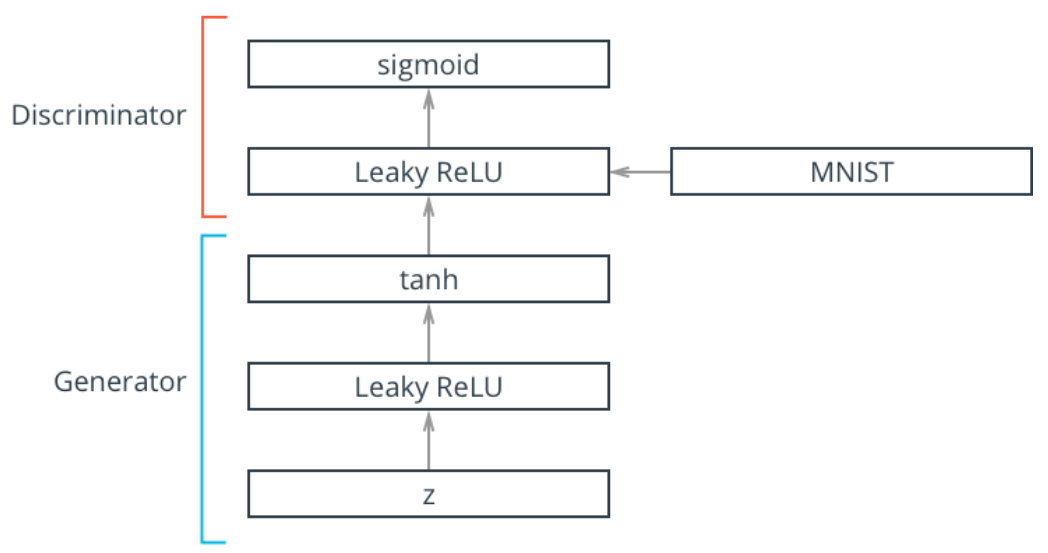
\includegraphics[width=0.6\textwidth,height=0.6\textheight,keepaspectratio]{images/simple_mnist.png}
    \captionsetup{justification=centering}
    \caption{GAN architecture for MNIST}
    \label{fig:f3}
\end{figure}

The discriminator loss can be denoted by Eq. \eqref{eq:1}. This loss is basically the sum of the losses for real and fake images. A real image as a label of 1 whereas a image generated by the generator has a label of 0.

\begin{equation}
Loss_D = Loss_{real} + Loss_{fake}
\label{eq:1}
\end{equation}

The generator loss is simply the loss of the Discriminator but flipped. Therefore, a generated image will have an output label of 1. This is done to fool the discriminator.

The training procedure of this network will involve alternating between training the discriminator and the generator. For the discriminator training the steps are:

\begin{itemize}
    \item Compute the discriminator loss on real, training images
    \item Generate fake images
    \item Compute the discriminator loss on fake, generated images
    \item Add up real and fake loss
    \item Perform backpropagation + an optimization step to update the discriminator's weights
\end{itemize}

Similarly, the training procedure for the generator is as follows:

\begin{itemize}
    \item Generate fake images
    \item Compute the discriminator loss on fake images, using flipped labels.
    \item Perform backpropagation + an optimization step to update the generator's weights
\end{itemize}

In \textit{DCGAN.ipynb} is an implementation of a Deep convolutional GAN. The main difference between this example and the last one is that now the discriminator and generator use convolutional neural networks. The discriminator architecture can be seen in Fig. \ref{fig:f4}.

\begin{figure}[ht]
    \centering
    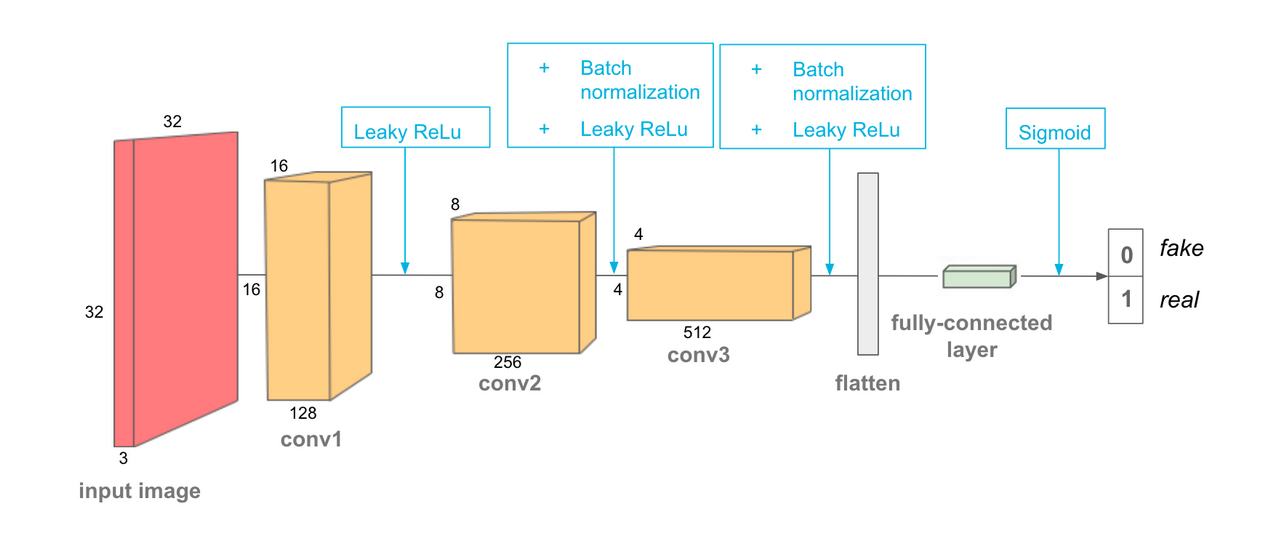
\includegraphics[width=0.75\textwidth,height=0.75\textheight,keepaspectratio]{images/discriminator.png}
    \captionsetup{justification=centering}
    \caption{Discriminator as a CNN}
    \label{fig:f4}
\end{figure}

Similarly, the generator network looks as shown by Fig. \ref{fig:f5}. It is important to mention that the first fully connected layer is used to increase the amount of parameters of the latent vector and then the output of the fully connected layer is reshaped into a set of feature maps with an specific depth to then be passed to the first transposed convolution and so on.

\begin{figure}[ht]
    \centering
    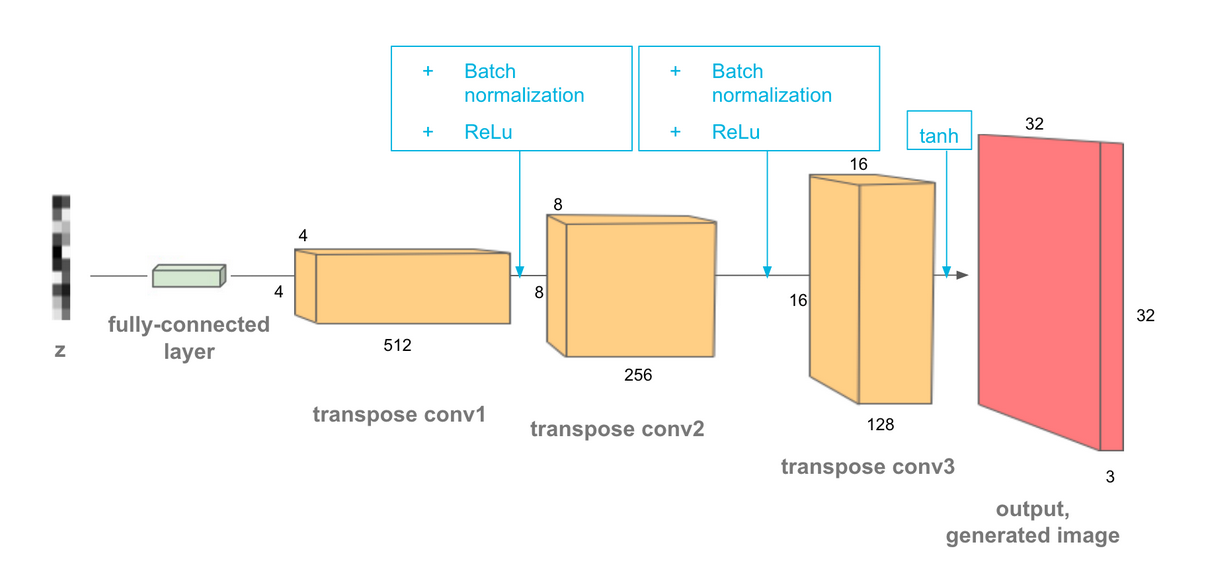
\includegraphics[width=0.75\textwidth,height=0.75\textheight,keepaspectratio]{images/generator.png}
    \captionsetup{justification=centering}
    \caption{Generator as a CNN}
    \label{fig:f5}
\end{figure}

Finally, in \textit{CycleGAN.ipynb} is an implementation of a Cycle Gan to map images from one domain to another. Further details are in the notebook and the implementation was done by udacity.

\printbibliography


\end{document}
